\documentclass[letterpaper,11pt]{article}

\usepackage[utf8]{inputenc}
\usepackage[left=2cm,right=2cm,top=2cm,bottom=2cm]{geometry} 
\usepackage[spanish,es-tabla]{babel}
\usepackage[table,xcdraw]{xcolor}

\usepackage{amssymb}
\usepackage{amsmath}
\usepackage{amsthm}
\usepackage{caption}
\usepackage{color}
%\usepackage{draftwatermark}
\usepackage{empheq}
\usepackage{fancyhdr}
\usepackage{fncychap}
\usepackage{float}
\usepackage{geometry}
\usepackage{graphicx}
\usepackage{hyperref}
\usepackage{mathrsfs}
\usepackage{multicol}
\usepackage{multirow}
\usepackage{mdframed}
\usepackage{booktabs}
\usepackage{lipsum}
\usepackage{graphicx}
\usepackage{color}
\usepackage{parskip}
\usepackage{psfrag}
\usepackage{pgfplots}
\usepackage{rotating}
\usepackage{siunitx}
\usepackage{subcaption}
\usepackage{bm}

\setlength{\parindent}{0pt}

\renewcommand{\arraystretch}{1.3}


\definecolor{ocre}{RGB}{243,102,25}
\definecolor{mygray}{RGB}{243,243,244}
\definecolor{deepGreen}{RGB}{26,111,0}
\definecolor{shallowGreen}{RGB}{235,255,255}
\definecolor{deepBlue}{RGB}{61,124,222}
\definecolor{shallowBlue}{RGB}{235,249,255}

%\SetWatermarkText{\textsc{--TR--}} 
%\SetWatermarkScale{5}
%\SetWatermarkColor{shallowBlue}
%\SetWatermarkAngle{90}

%\pagestyle{fancy}
%\lhead{ddd}
%\rhead{ssss}
%\cfoot{\thepage}

%\usepackage{fontspec}
%\setmainfont{Arial}
\usepgfplotslibrary{colorbrewer}
\pgfplotsset{width=8cm,compat=1.9}

\begin{document}
	\begin{titlepage}
		\centering
	
		{\scshape\huge Instituto Politécnico Nacional \par}
		\vspace{1cm}
		{\scshape\Large Escuela Superior de Cómputo \par}
		\vspace{0.3cm}
		Ciudad de México, México,  7 de marzo de 2024.
	
		\vfill
	
		%TITULO:
		{\huge\bfseries Práctica 1 \par}
	
		\vfill
	
		{\large García Carrizoza André  202363AAAA \par}
		
		{\large Juarez Leyva Jorge Antonio  2020330111\par}
		\vspace*{0.5cm}
		%MATERIA:
		{\large Fundamentos de Inteligencia Artificial}\par
		%PROFESOR
		{\large Hernández Cruz Macario}\par
		%Grupo
		\vfill
	
	\end{titlepage}
	\section{Resumen}
En este documento se presenta el desarrollo de una aplicación con dos agentes, que se encuentran en un entorno bidimensional con muestras y obstáculos, los agentes desempeñan la tarea de las muestras, moviéndose de manera aleatoria, y llevarlas a la base, por el camino con distancia \textit{manhattan} más corta, en ambos casos deben esquivar los obstáculos que se encuentran en el entorno. 
	\section{Introducción}


	\section{Desarrollo}
	\section{Funcionamiento}
	La figura \ref*{figInitialState} muestra el estado de la aplicación al abrir, lso agentes se colocan de manera aleatoria en el entorno, para colocar los objetos, en el menú superior se encuentran las opciones. Para colocar un objeto basta con dar click en la opción deseada y luego dar click en el tablero.
	
	Una vez se colocan todos los elementos la aplicación luce como en la figura \ref*{figSetUp}, luego se selecciona la opción de \textit{file} en el menú superior y se da click en \textit{run} para que los agentes desarrollen su tarea.
	
	Cuando un agente tiene una muestra se dirige a la nave por la distancia más corta, como se muestra en la figura \ref*{figSample} saltándose cualquier otra muestra que pueda estar en el camino. Una ver terminado el tablero queda sin muestras (figura \ref*{figEnd}).
	
	\begin{multicols}{2}
		\begin{figure}[H]
			\centering
			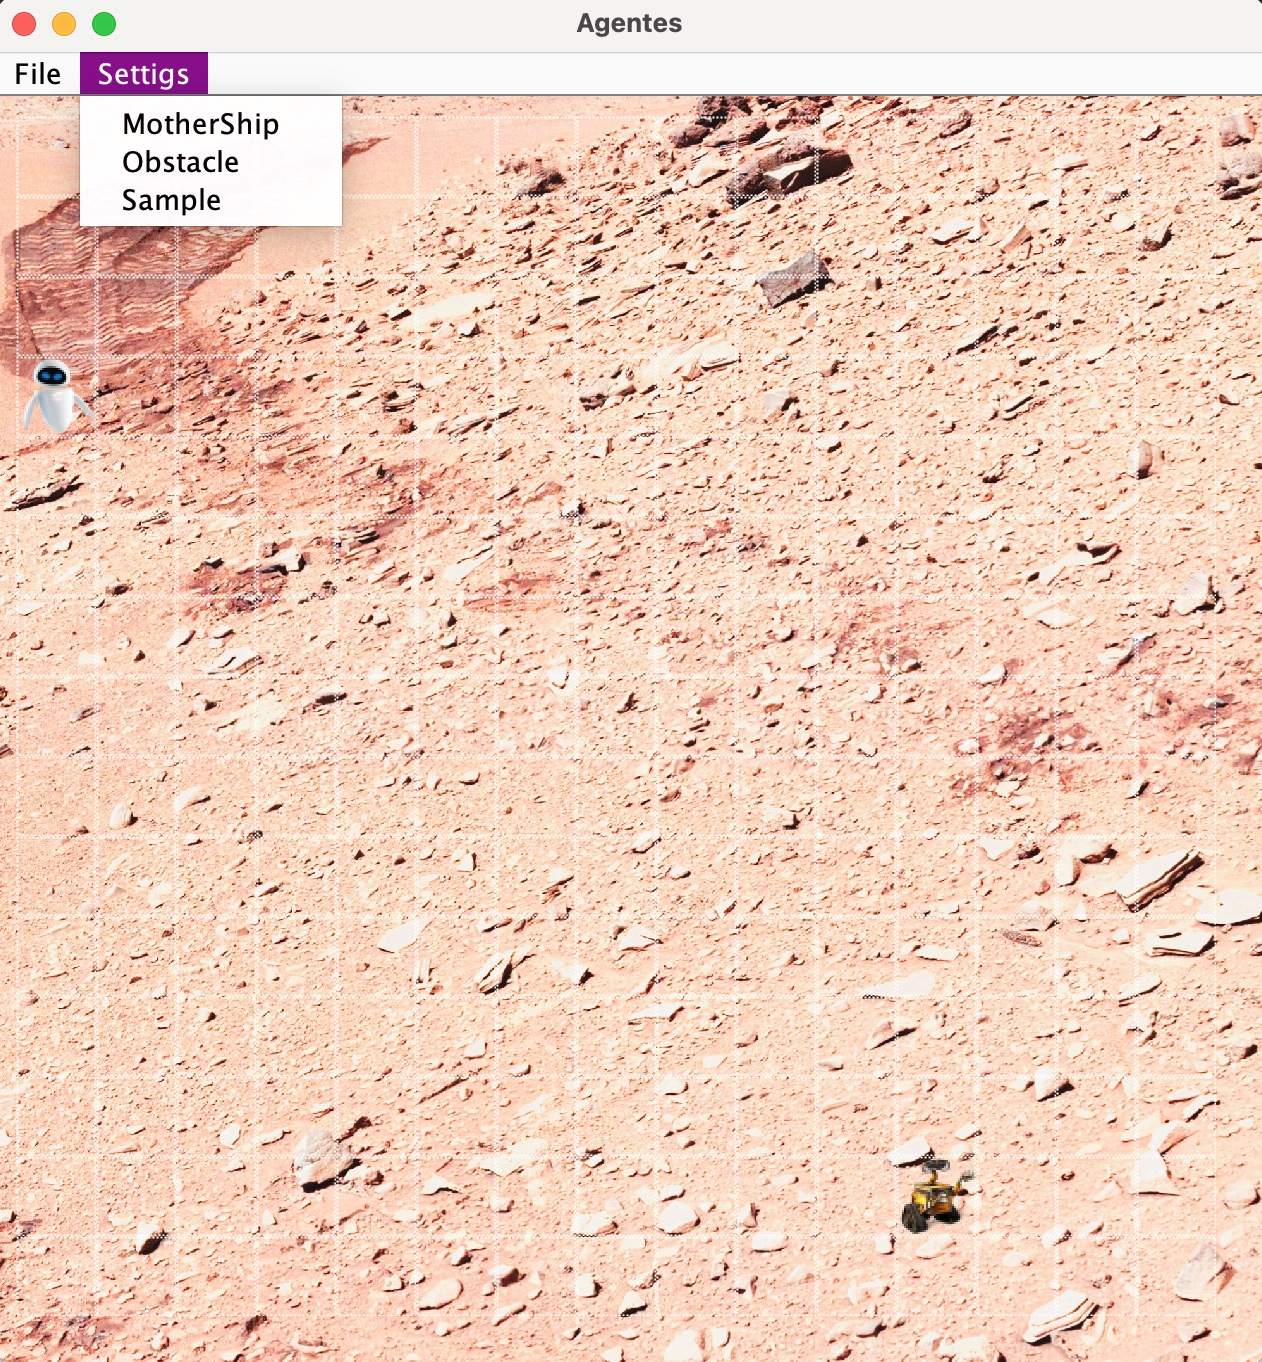
\includegraphics[width = 5cm]{images/initialState.jpg}
			\caption{Estado inicial de la aplicación.}
			\label{figInitialState}
		\end{figure}
		
	
		\begin{figure}[H]
			\centering
			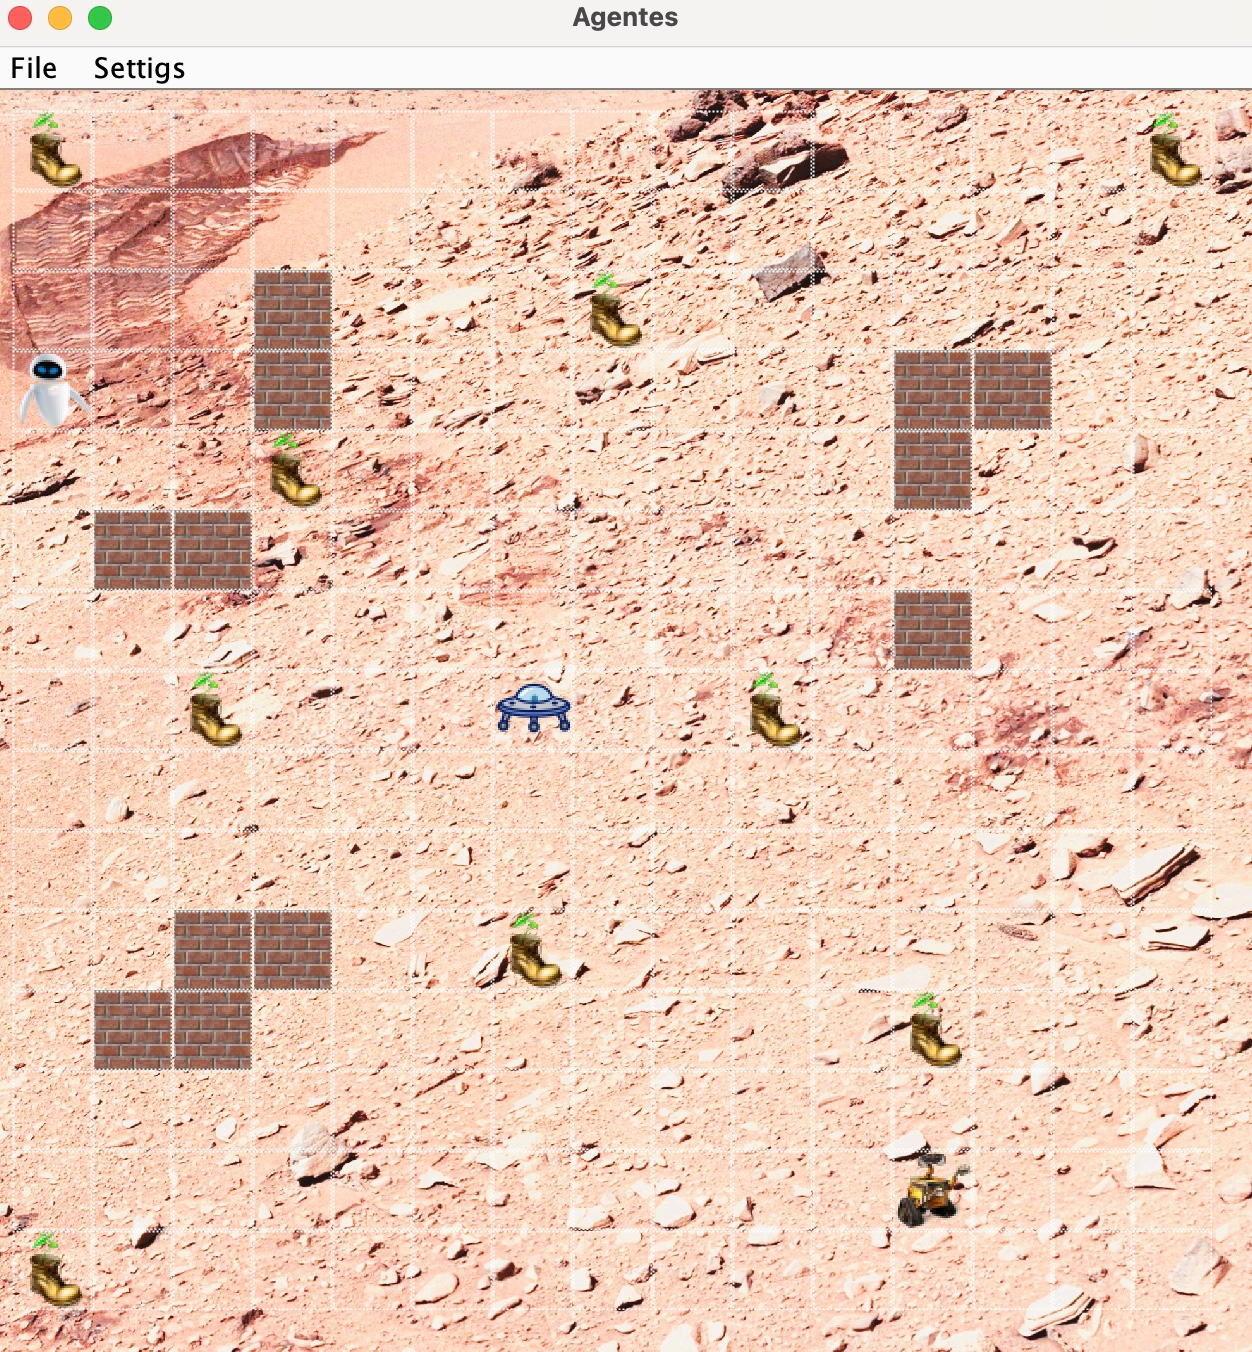
\includegraphics[width = 5cm]{images/setUp.jpg}
			\caption{Se configuró el entorno agregando la nave, las muestras y los obstáculos.}
			\label{figSetUp}
		\end{figure}
		
		\begin{figure}[H]
			\centering
			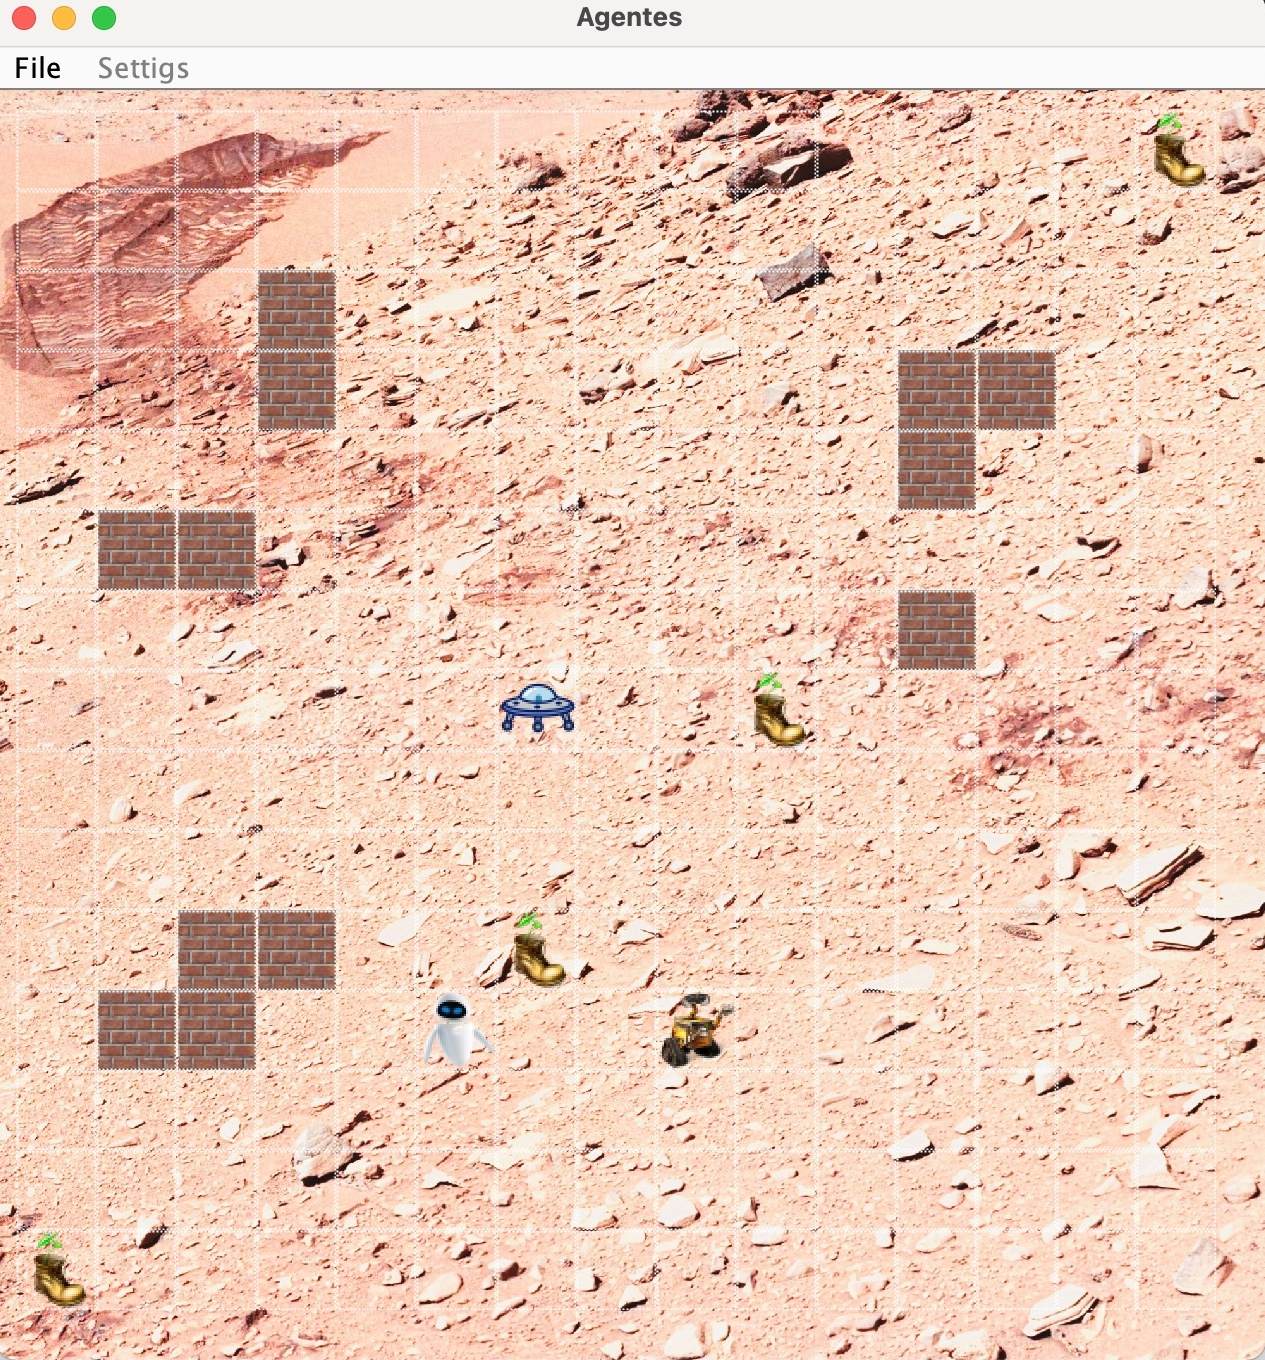
\includegraphics[width = 5cm]{images/sample.jpg}
			\caption{El agente dos se dirige a la nave por la distancia \textit{manhattan} más corta.}
			\label{figSample}
		\end{figure}
		\begin{figure}[H]
			\centering
			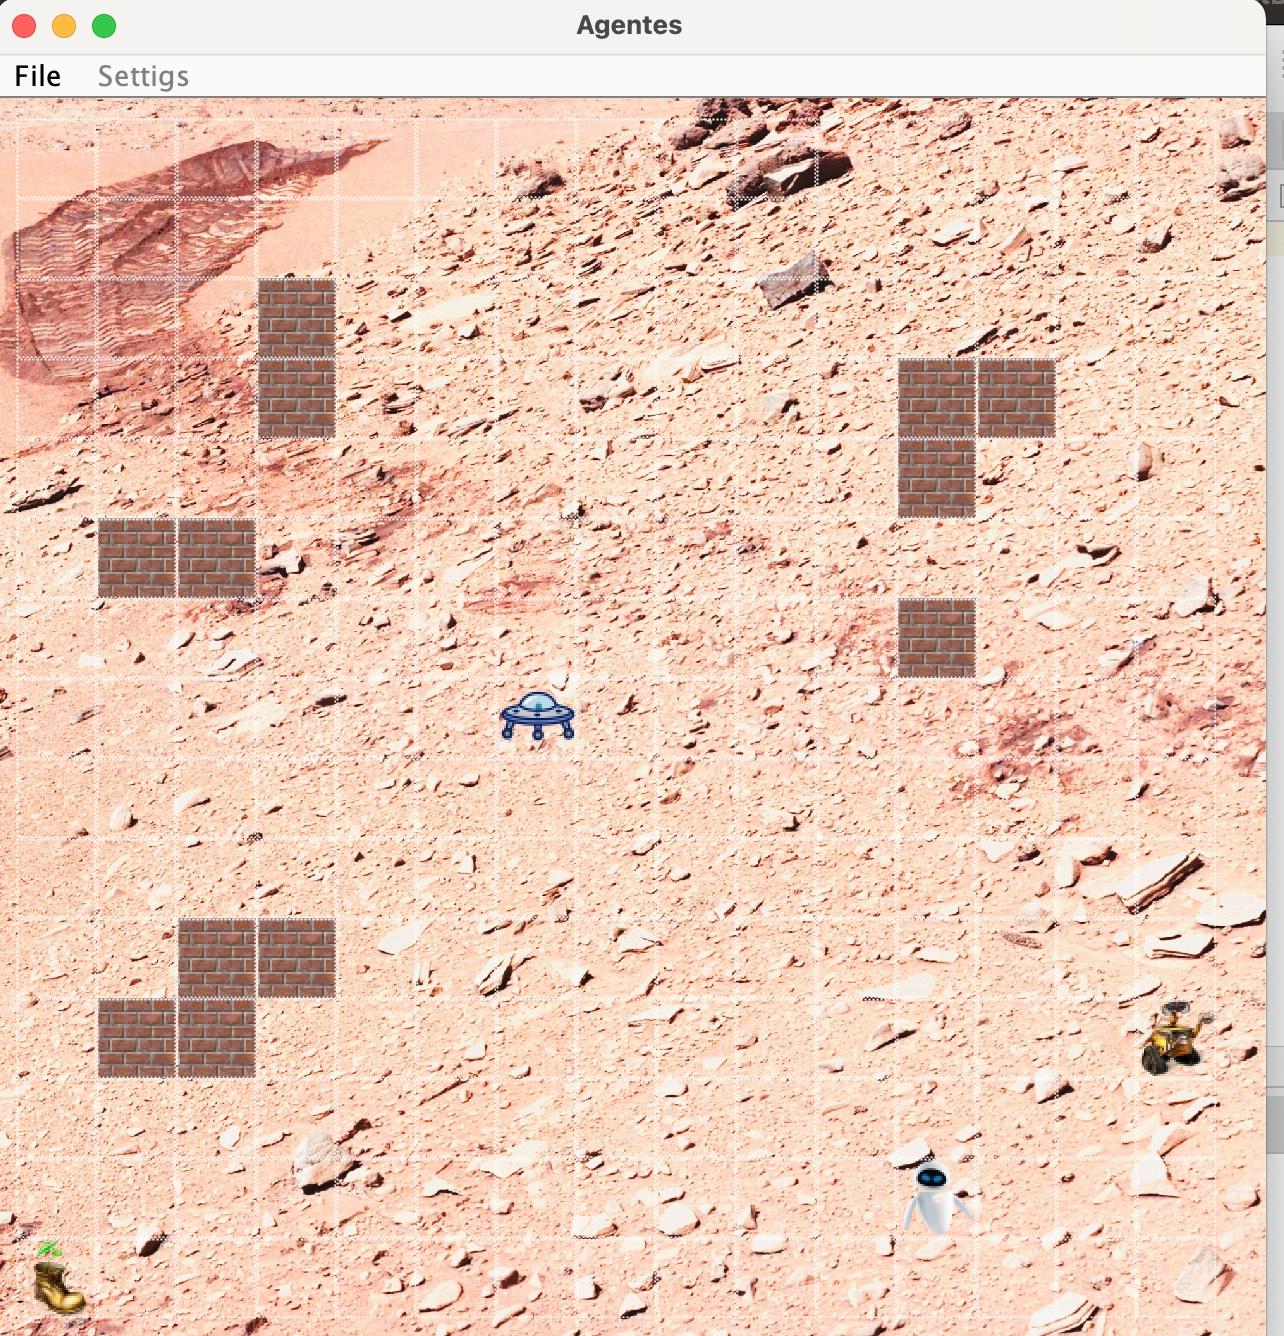
\includegraphics[width = 5cm]{images/end.jpg}
			\caption{Los agentes recolectaron todas las muestras.}
			\label{figEnd}
		\end{figure}
	\end{multicols}
	\section{Conclusiones}
Con la implementación de los agentes se reforzaron los conocimientos adquiridos en paradigmas de programación, con la implementación de funciones y clases anónimas para facilitar el desarrollo del movimiento de los agentes, los cuales cumplieron exitosamente la función de recoger las muestras y llevarlas a la nave, ambos de manera independiente. 
	\section{Bibliografia}
\end{document}